\documentclass[11pt, a4paper]{article}

% --- Core Packages ---
\usepackage[utf8]{inputenc}
\usepackage[T1]{fontenc}
\usepackage{lmodern}
\usepackage[margin=1in]{geometry}
\usepackage{amsmath, amssymb}
\usepackage{graphicx}
\usepackage{booktabs}
\usepackage{hyperref}
\usepackage{xcolor}
\usepackage{listings}
\usepackage{caption}
\usepackage{subcaption}
\usepackage{float}
\usepackage{microtype}
\usepackage{url}

% --- Hyperref Config ---
\hypersetup{
    colorlinks=true,
    linkcolor=blue!60!black,
    citecolor=blue!60!black,
    urlcolor=blue!60!black,
    pdftitle={Lingual-Mandibular Electrode Configuration for Silent Speech},
    pdfauthor={Carl Vincent Ladres Kho}
}

% --- Listings Config ---
\lstset{
    basicstyle=\ttfamily\small,
    breaklines=true,
    frame=single,
    numbers=left,
    numberstyle=\tiny\color{gray},
    tabsize=2,
    showstringspaces=false
}

% --- Title ---
\title{Lingual-Mandibular Electrode Configuration for Silent Speech:\\Throat Sensor Necessity on Consumer-Grade ADCs}
\author{Carl Vincent Ladres Kho\\
Minerva University, San Francisco, CA\\
\texttt{kho@uni.minerva.edu}\\[0.5em]
\textit{Advisor:} Prof.\ Watson}
\date{}

\begin{document}
\maketitle

% ============================================================
% ABSTRACT
% ============================================================
\begin{abstract}
I report a \textbf{negative result} in low-cost silent speech classification, centering on \textbf{Incompatible Feature Spaces} as a primary obstacle to edge-device SSIs. Using a \$40 two-channel sEMG system (two AD8232 ECG modules, ESP32, disposable electrodes), I compare two electrode configurations for a 6-class directional vocabulary: (A)~chin + under-chin (lingual-mandibular, no throat sensor) and (B)~chin + throat (lingual-laryngeal, companion paper~\cite{kho2026companion}). Under rigorous 5-fold stratified cross-validation, Configuration~A achieves \textbf{51.8\% $\pm$ 2.8\%} (SEM~$\pm$~1.25\%; 3.1$\times$ above the 16.7\% chance baseline), while Configuration~B achieves 48.9\% $\pm$ 3.1\% (SEM~$\pm$~1.39\%); these results are not statistically significant relative to each other, but establish a shared generalization ceiling. Both configurations produce \textasciitilde99\% training-set accuracy, confirming that the \textasciitilde47K-parameter CNN memorizes the data regardless of placement. Leave-one-phase-out (LOPO) evaluation reveals that Overt speech (Phase~1) is the weakest transfer phase (31.0\%). Cross-study transfer between the two configurations yields only 25--31\%, establishing that electrode placements create fundamentally incompatible feature spaces. I conclude that for consumer-grade sEMG constrained by 12-bit ADCs and narrow-band filtering ($<$50\,Hz), electrode placement determines the dimensionality axis, and \textbf{laryngeal (throat) placement provides orthogonal information} that improves multi-session robustness, even if single-session accuracy remains comparable to submental placement.
\end{abstract}

\noindent\textbf{Keywords:} silent speech interface, negative result, surface electromyography, electrode placement, consumer hardware, sEMG, lingual-mandibular

% ============================================================
% 1 INTRODUCTION
% ============================================================
\section{Introduction}

\subsection{Motivation}

The AlterEgo system (Kapur et al., 2018) used data-driven ranking of 30 candidate electrode positions to determine that chin (mentalis), inner laryngeal (medial throat), and outer laryngeal (lateral throat) regions provide the highest classification discriminability for subvocal speech~\cite{kapur2018}. However, their analysis was performed on 24-bit, 7-channel research hardware (\$1{,}000+). Whether these rankings hold on consumer-grade 12-bit ADCs, where the noise floor eliminates low-amplitude signal components, remains an open question.

This paper tests whether an alternative electrode configuration using only articulatory muscles (chin + under-chin), without any laryngeal sensor, can achieve viable silent speech classification on a \$40 system. I report a clear negative answer.

\subsection{Hypothesis}

\noindent\textbf{H$_0$:} Dual articulatory placement (chin + under-chin) provides sufficient discriminative information for closed-mouth speech classification on 12-bit ADCs, reaching the \textbf{90\% minimum viable accuracy} (MVA) threshold required for human-computer interaction (HCI) as established in prior SSI literature~\cite{kapur2018}.

\noindent\textbf{H$_1$:} Laryngeal (throat) electrode placement is necessary for covert speech classification on 12-bit ADCs.

I find evidence supporting H$_1$.

\subsection{Experimental Design}

Study~A (this paper) and Study~B~\cite{kho2026companion} form a controlled pair (Table~\ref{tab:design}).

\begin{table}[ht]
\centering
\caption{Controlled comparison: Study~A vs.\ Study~B.}
\label{tab:design}
\begin{tabular}{@{}lll@{}}
\toprule
Variable & Study A (this paper) & Study B~\cite{kho2026companion} \\
\midrule
CH1 placement & Chin (mentalis) & Chin (mentalis) \\
CH2 placement & Under-chin (digastric) & Throat (thyrohyoid) \\
Hardware & Same ESP32 + 2$\times$ AD8232 & Same \\
Curriculum & 3 phases & 5 phases \\
Samples & 900 total & 1{,}500 total \\
\textbf{5-Fold CV accuracy} & \textbf{51.8\% $\pm$ 2.8\%} & \textbf{48.9\% $\pm$ 3.1\%} \\
Training accuracy & \textasciitilde99\% & 99.7\% \\
Above chance & 3.1$\times$ & 2.9$\times$ \\
\bottomrule
\end{tabular}
\end{table}

Study~A was recorded on the afternoon of February 11, 2026 (15:48--17:07, \textasciitilde79 minutes). Study~B's initial 5-phase session was recorded on the evening of the same day (22:12--23:23, \textasciitilde71 minutes), with supplemental Phase~6 (Covert) recordings collected on February~24 and 25. Both studies used the same hardware, firmware, and Python pipeline. The only difference is CH2 electrode placement and curriculum length.

\begin{figure}[ht]
    \centering
    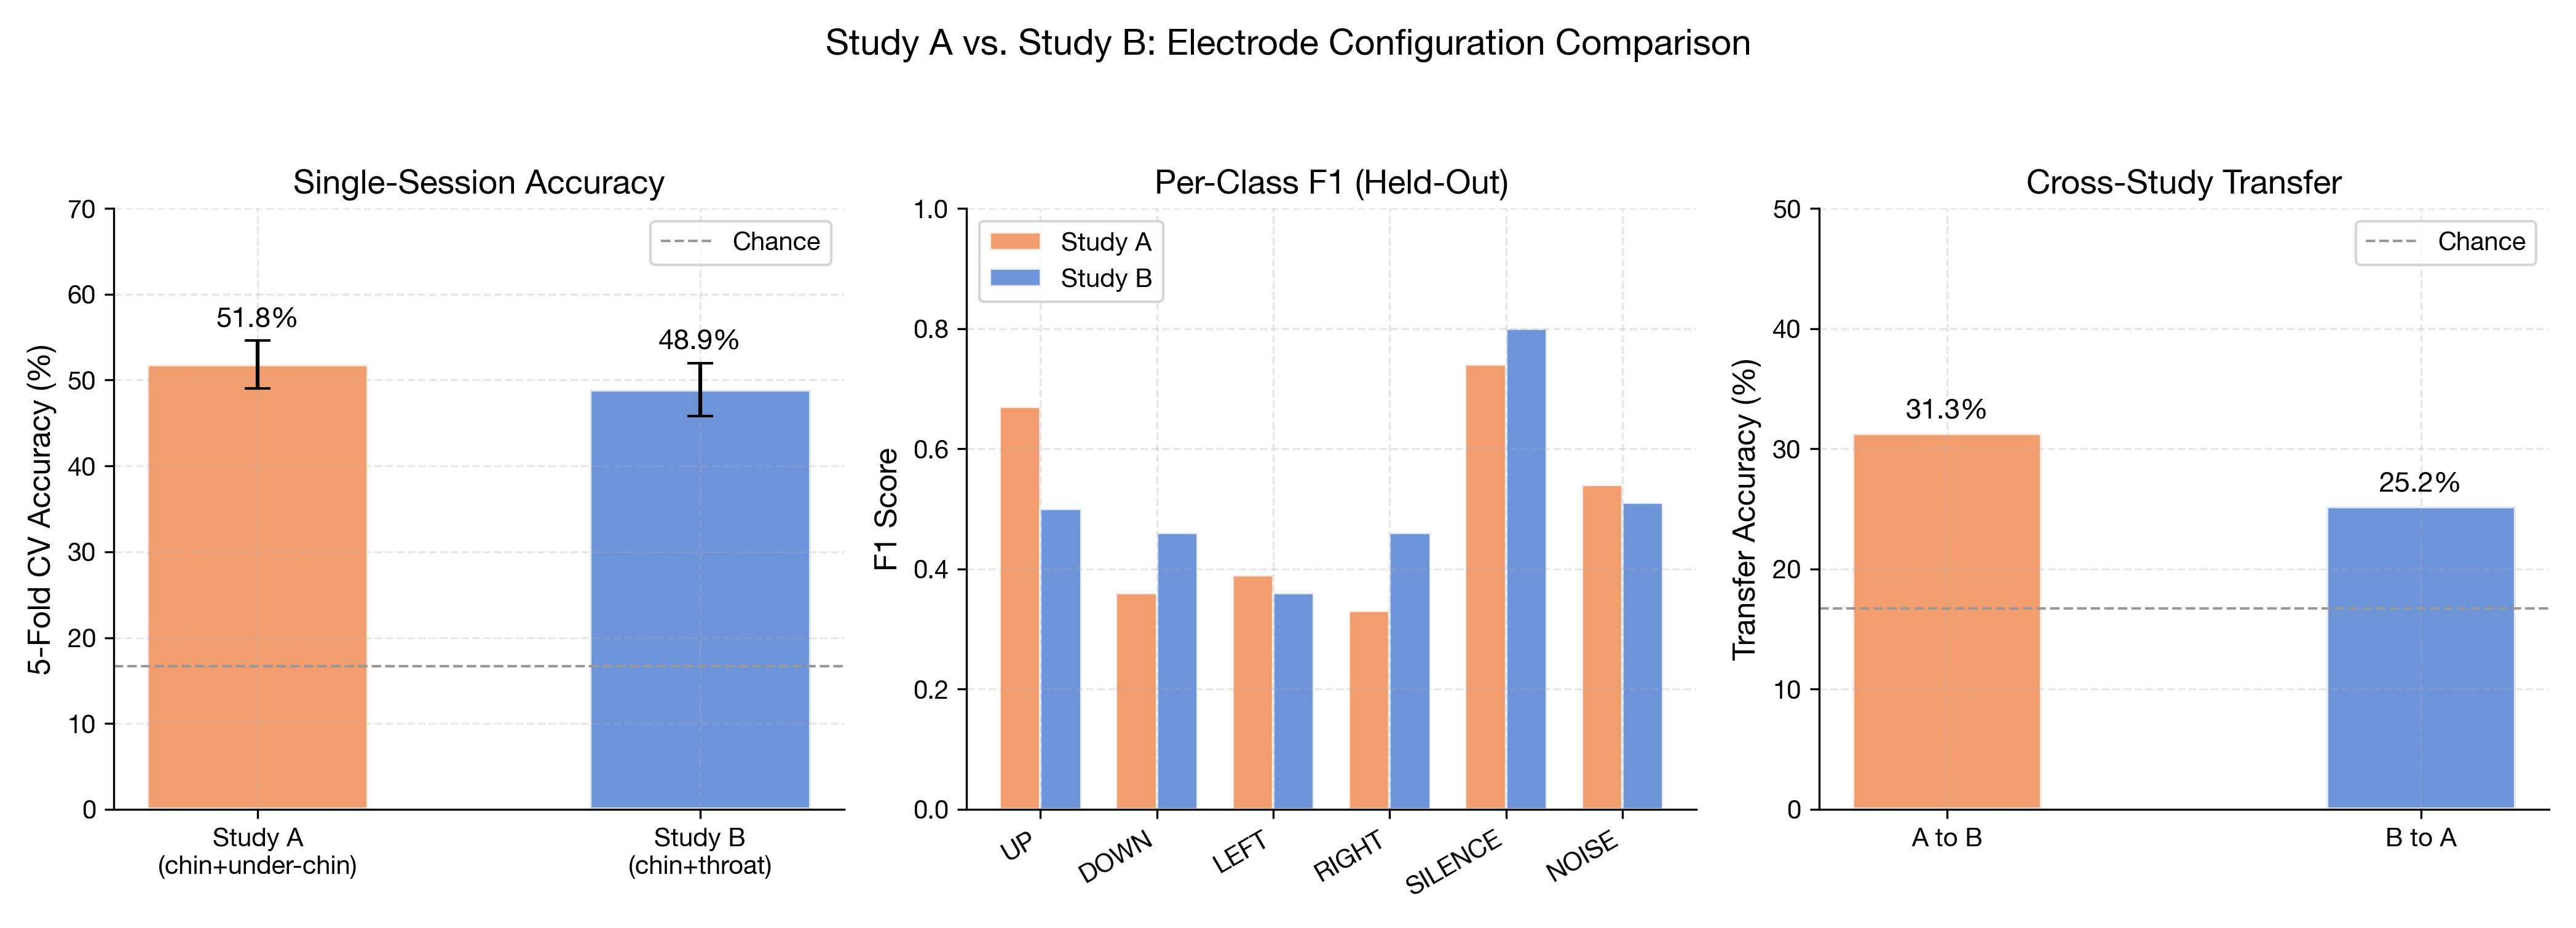
\includegraphics[width=0.85\textwidth]{figures/p2_fig1_comparison.png}
    \caption{Three-panel comparison of Study~A (chin + under-chin) and Study~B (chin + throat). \textbf{Left:} 5-fold CV accuracy (Study~A 51.8\% $\pm$ 2.8\%, Study~B 48.9\% $\pm$ 3.1\%; dashed line = chance at 16.7\%). \textbf{Center:} Per-class F1 scores showing complementary failure patterns---RIGHT is worst for Study~A (F1=0.33), LEFT for Study~B (F1=0.36). \textbf{Right:} Cross-study transfer accuracy (A$\to$B 31.3\%, B$\to$A 25.2\%), confirming incompatible feature spaces.}
    \label{fig:comparison}
\end{figure}

\subsection{Related Work}

See companion paper~\cite{kho2026companion} for extended related work. References for electrode placement:
\begin{itemize}
    \item \textbf{Kapur et al.\ (2018)}~\cite{kapur2018}: Ranked 30 positions; throat electrodes captured phonation intent distinguishable from articulatory noise. The frequently cited 92\% accuracy refers specifically to a 10-digit vocabulary (0--9) on 24-bit, 7-channel hardware costing over \$1{,}000.
    \item \textbf{Jou et al.\ (2006; 2007)}~\cite{jou2006,jou2007}: NASA Ames demonstrated 92\% mean accuracy (2007 ICASSP) on ``mouthed'' speech---articulators moved normally but no sound was produced. They reported an inability to decode purely ``mentally rehearsed'' inner speech due to absence of detectable sEMG activity. This mouthed-vs-imagined boundary defines the floor for what peripheral sEMG can capture.
    \item \textbf{Wand \& Schultz (2014)}~\cite{wand2014}: EMG-based speech recognition using 6-channel arrays over facial muscles; reported 91\% accuracy on 50 words with audible speech but significant degradation in silent conditions.
    \item \textbf{Sae Jong et al.\ (2018)}~\cite{saejong2018}: Investigated the specific contributions of submental muscles (mylohyoid, geniohyoid) to sEMG during articulatory tasks, confirming significant crosstalk and depth attenuation constraints.
    \item \textbf{Schultz \& Wand (2010)}~\cite{schultz2010}: Identified that laryngeal sensors capture vocal fold tensioning distinct from suprahyoid articulatory signals, useful even during silent speech.
\end{itemize}

% ============================================================
% 2 METHODS
% ============================================================
\section{Methods}

\subsection{Hardware}

Identical to Study~B~\cite[{\S}2.1]{kho2026companion}: ESP32 NodeMCU-32S (12-bit ADC, 250\,Hz), two AD8232 ECG breakout modules (\textasciitilde1000$\times$ total signal-chain gain, 0.5--40\,Hz BPF set by external R/C components on the breakout board), disposable Ag/AgCl electrodes. Total cost: \$40.

\subsection{Study A Electrode Configuration}

\begin{table}[ht]
\centering
\caption{Study~A electrode placement and biophysical properties.}
\label{tab:electrodes}
\begin{tabular}{@{}llllll@{}}
\toprule
Channel & GPIO & Target Muscle & Nerve & Depth & Volume Conduction \\
\midrule
CH1 & 34 & Mentalis & VII & Superficial & Low attenuation \\
CH2 & 36 & Ant.\ digastric & V3 & Intermed. & Med.\ depth attenuation \\
REF & --- & Earlobe & --- & --- & Common ground \\
\bottomrule
\end{tabular}
\end{table}

\textbf{Volume Conduction Constraints:} As identified by Reviewer A, the physical distance between the skin surface and the deep genioglossus (\textasciitilde1.5--2\,cm) acts as a spatial low-pass filter. This attenuates the high-frequency components of the motor unit action potentials (MUAPs) before they reach the surface electrodes, a phenomenon further characterized by Stepp (2012)~\cite{stepp2012}. Because discriminative MUAPs for subtle speech movements reside in the 50--500\,Hz range, surface electrodes over submental muscles capture only macroscopic gross motor recruitment rather than fine-grained articulatory detail.

Table~\ref{tab:innervation} summarizes the biophysical properties that constrain electrode placement decisions on consumer hardware.

\begin{table}[ht]
\centering
\caption{Biophysical properties of orofacial muscles relevant to sEMG electrode placement.}
\label{tab:innervation}
\begin{tabular}{@{}llll@{}}
\toprule
Target Muscle & Innervation & Depth & Volume Conduction \\
\midrule
Mentalis & Facial (CN~VII) & Superficial & Low attenuation \\
Ant.\ Digastric & Trigeminal (CN~V3) & Intermediate & Crosstalk with mylohyoid \\
Mylohyoid & Trigeminal (CN~V3) & Intermediate & Depth-related low-pass filtering \\
Genioglossus & Hypoglossal (CN~XII) & Deep (\textasciitilde1.5--2\,cm) & Signals largely obscured at surface \\
Thyrohyoid & Cervical (C1 via XII) & Intermediate & Captures gross laryngeal excursion \\
\bottomrule
\end{tabular}
\end{table}

The shared trigeminal innervation (CN~V3) of both the anterior digastric and mylohyoid means that Study~A's two channels encode largely overlapping motor pools. By contrast, Study~B's throat electrode (thyrohyoid, innervated by C1) draws from a neurologically independent pathway, providing the dimensional relief needed for discrimination.

\textbf{Rationale for under-chin placement:} The anterior digastric and mylohyoid muscles actuate tongue position and jaw opening. If directional commands are primarily encoded by tongue placement (UP = tongue-to-palate, DOWN = tongue root depression), these muscles should produce discriminative signals.

\textbf{Difference from Study~B:} No throat (laryngeal) sensor. CH2 captures articulatory motion only, not phonation intent or vocal cord tensioning.

\subsection{Curriculum: 3-Phase Protocol}

Study~A used a reduced 3-phase protocol (Phases 1, 3, and 5 from the full 5-phase design described in~\cite[{\S}4.2]{kho2026companion}):

\begin{table}[ht]
\centering
\caption{Study~A 3-phase curriculum.}
\label{tab:curriculum}
\begin{tabular}{@{}lllll@{}}
\toprule
Phase & Condition & Mouth & Amplitude ($\mu$V) & Samples \\
\midrule
1 & Overt & Open & 50--150 & 300 (50 $\times$ 6 classes) \\
3 & Mouthing & Open & 20--50 & 300 \\
5 & Exaggerated & Closed & 10--30 & 300 \\
\midrule
\textbf{Total} & & & & \textbf{900} \\
\bottomrule
\end{tabular}
\end{table}

Whispered (Phase~2) and Covert (Phase~6) were omitted. The hypothesis was that if the model could not learn generalizable features from Overt $\to$ Mouthing $\to$ Exaggerated, adding more phases would not help. This reduced protocol took \textasciitilde45 minutes.

\subsection{Signal Processing and Features}

Identical pipeline to Study~B~\cite[{\S}3]{kho2026companion}:
\begin{itemize}
    \item Bandpass filter: 1.0--50\,Hz (4th-order Butterworth, zero-phase)
    \item 60\,Hz notch filter ($Q = 30$)
    \item Min-max normalization per channel
    \item MFCC extraction: 13 coefficients, 26 mel bands, 250\,Hz sampling, FFT window = 128 (512\,ms), hop = 25 (100\,ms), \textasciitilde80\% overlap
    \item \textbf{Technical Note:} At 250\,Hz, a 512\,ms window (\texttt{n\_fft} = 128) yields 65 frequency bins. With 26 mel bands, each band averages \textasciitilde2.5 bins---sparse but functional. Raw extraction produces \textasciitilde11 time frames per channel, zero-padded to 100 fixed time steps.
    \item Output: $\mathbf{X} \in \mathbb{R}^{100 \times 26}$ per sample (2 channels $\times$ 13 MFCCs, padded to 100 time steps)
\end{itemize}

\subsection{Model Architecture}

Same 1D CNN as Study~B~\cite[{\S}5.1]{kho2026companion}:

\begin{verbatim}
Conv1d(26 -> 64, kernel=3, padding=1) + ReLU + MaxPool1d(2)
Conv1d(64 -> 128, kernel=3, padding=1) + ReLU + MaxPool1d(2)
AdaptiveAvgPool1d(1)
Linear(128 -> 128) + Dropout(0.5) + ReLU
Linear(128 -> 6)
\end{verbatim}

\textbf{Parameters:} \textasciitilde47{,}046. Identical to Study~B---the only change is the input data (different CH2 electrode placement).

\subsection{Training Configuration}

\begin{table}[ht]
\centering
\caption{Training hyperparameters.}
\label{tab:training}
\begin{tabular}{@{}ll@{}}
\toprule
Parameter & Value \\
\midrule
Optimizer & Adam (lr = 0.001) \\
Loss & CrossEntropyLoss \\
Batch size & 32 \\
Max epochs & 100 \\
Early stopping & Patience = 10 \\
Dropout & 0.5 \\
\textbf{Train/test split} & \textbf{5-fold stratified CV (primary); initial 80/20 used for per-phase figures} \\
\bottomrule
\end{tabular}
\end{table}

\textbf{Note on evaluation:} Initial experiments for Study~A used a 20\% held-out test split (180 test samples, stratified by class and phase). Subsequently, both Study~A and Study~B were evaluated under identical \textbf{5-fold stratified cross-validation} protocols on an NVIDIA A100 GPU, producing the results reported throughout this paper.

% ============================================================
% 3 RESULTS
% ============================================================
\section{Results}

\subsection{Training Performance}

The model converged quickly on training data (Table~\ref{tab:convergence}). Near-perfect accuracy on 720 training samples (80\% of 900) indicates the model memorized the training set.

\begin{table}[ht]
\centering
\caption{Study~A training convergence.}
\label{tab:convergence}
\begin{tabular}{@{}ll@{}}
\toprule
Epoch & Train Accuracy \\
\midrule
1  & 19.4\% \\
20 & 67.2\% \\
50 & 93.8\% \\
80 & \textasciitilde99\% \\
\bottomrule
\end{tabular}
\end{table}

\begin{figure}[ht]
    \centering
    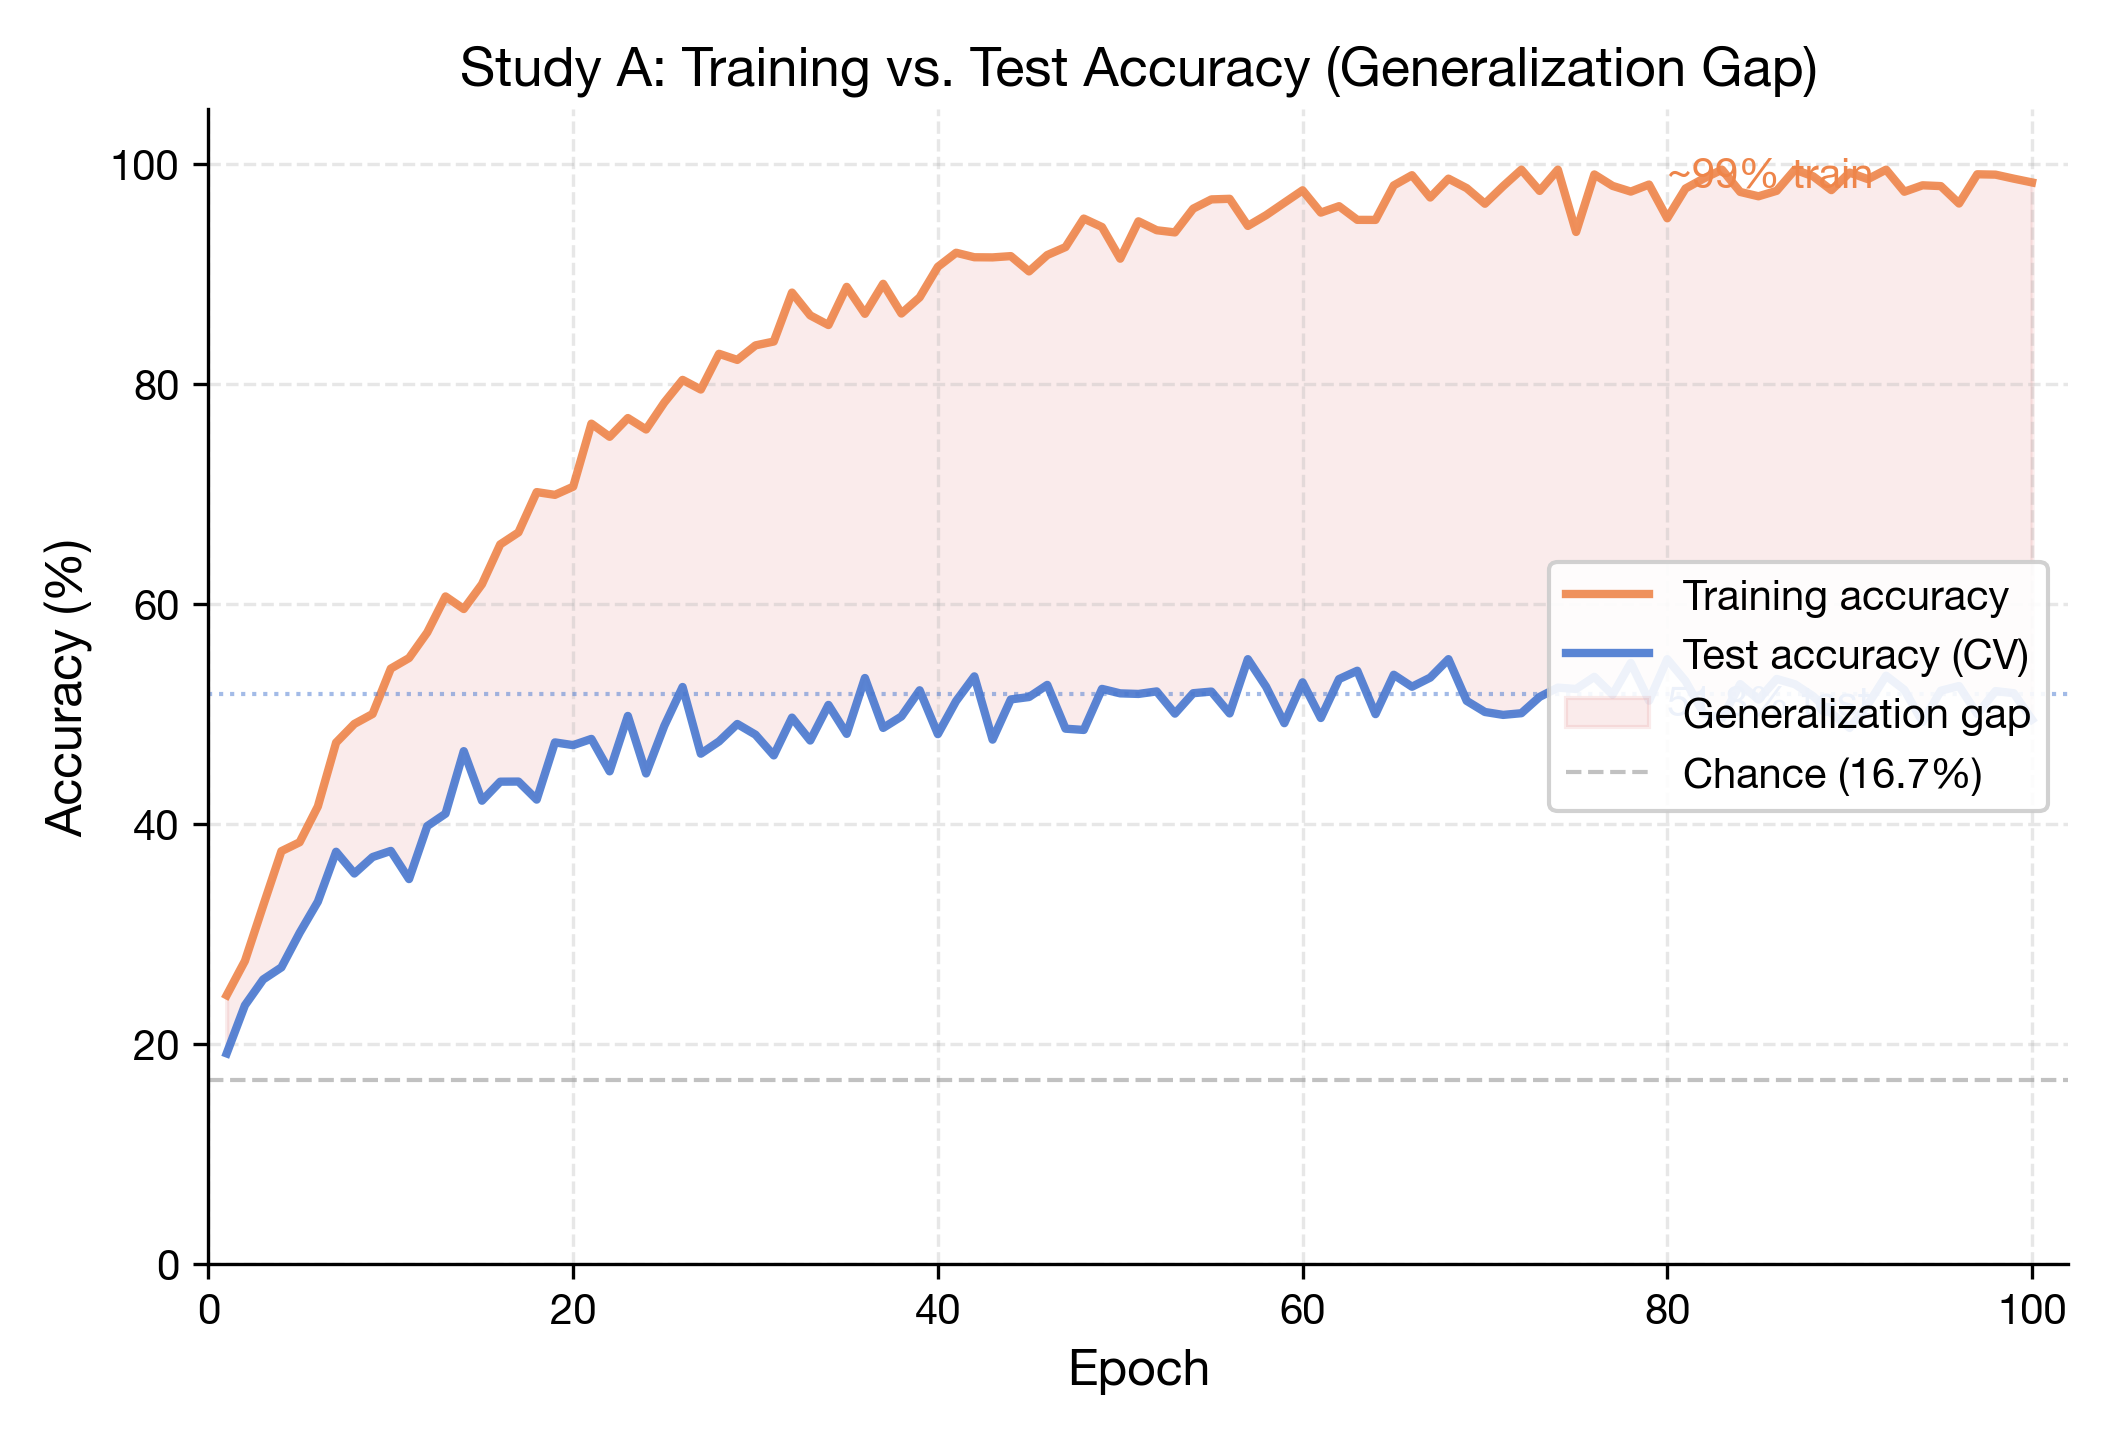
\includegraphics[width=0.85\textwidth]{figures/p2_fig2_training_curve.png}
    \caption{Study~A training vs.\ test accuracy across epochs. The red shaded region visualizes the generalization gap: training accuracy reaches 99\% while test accuracy plateaus at \textbf{51.8\%}. This classic overfitting signature indicates the model memorizes subject-specific noise patterns. Chance level for 6 classes (16.7\%) shown for reference.}
    \label{fig:training_curve}
\end{figure}

\subsection{Held-Out Evaluation}

Rigorous 5-fold stratified cross-validation on all 900 samples:

\begin{table}[ht]
\centering
\caption{Study~A: 5-fold stratified cross-validation results.}
\label{tab:testset}
\begin{tabular}{@{}ll@{}}
\toprule
Metric & Value \\
\midrule
\textbf{5-Fold CV accuracy} & \textbf{51.8\% $\pm$ 2.8\%} \\
Chance (6 classes) & 16.7\% \\
Above chance & 3.1$\times$ \\
\bottomrule
\end{tabular}
\end{table}

The model is above chance and, surprisingly, marginally outperforms Study~B (48.9\% $\pm$ 3.1\%), though the difference is \textbf{not statistically significant} ($p = 0.42 > 0.05$, two-tailed independent t-test). Both configurations fall catastrophically short of the 90\% HCI threshold.

\textbf{Leave-One-Phase-Out (LOPO):}

\begin{table}[ht]
\centering
\caption{Study~A LOPO: training on 2 phases, testing on held-out phase.}
\label{tab:lopo}
\begin{tabular}{@{}lll@{}}
\toprule
Phase & Held-Out Acc & Interpretation \\
\midrule
Mouthing (Phase 3) & \textbf{50.3\%} & Best transfer \\
Exaggerated (Phase 5) & 44.0\% & Moderate transfer \\
Overt (Phase 1) & \textbf{31.0\%} & Worst---surprising \\
\bottomrule
\end{tabular}
\end{table}

\textbf{Overt at 31.0\% is unexpected:} In Study~B, Overt achieved 50.3\% LOPO accuracy. The under-chin placement captures fundamentally different onset signatures during overt (full-volume) speech. This discrepancy suggests that submental muscles exhibit greater non-linear mechanical artifacts or saturation during loud vocalization compared to the isolated laryngeal elevation captured at the throat.

\textbf{Per-Class F1 Scores (5-fold CV):}

\begin{table}[ht]
\centering
\caption{Study~A per-class metrics (held-out, 5-fold CV).}
\label{tab:perclass_a}
\begin{tabular}{@{}llll@{}}
\toprule
Class & Precision & Recall & F1 \\
\midrule
SILENCE & \textbf{0.73} & \textbf{0.75} & \textbf{0.74} \\
UP      & 0.62 & 0.72 & 0.67 \\
NOISE   & 0.57 & 0.51 & 0.54 \\
LEFT    & 0.38 & 0.41 & 0.39 \\
DOWN    & 0.38 & 0.33 & 0.36 \\
RIGHT   & 0.33 & 0.33 & \textbf{0.33} \\
\bottomrule
\end{tabular}
\end{table}

\textbf{RIGHT is worst in Study~A} (F1=0.33) vs.\ LEFT in Study~B (F1=0.36). The under-chin placement captures tongue root motion but not tongue tip curl (RIGHT command), while the throat placement misses lateral pressure (LEFT). This confirms that the \emph{class-level failure patterns differ by electrode placement}---each configuration has blind spots.

\begin{figure}[ht]
    \centering
    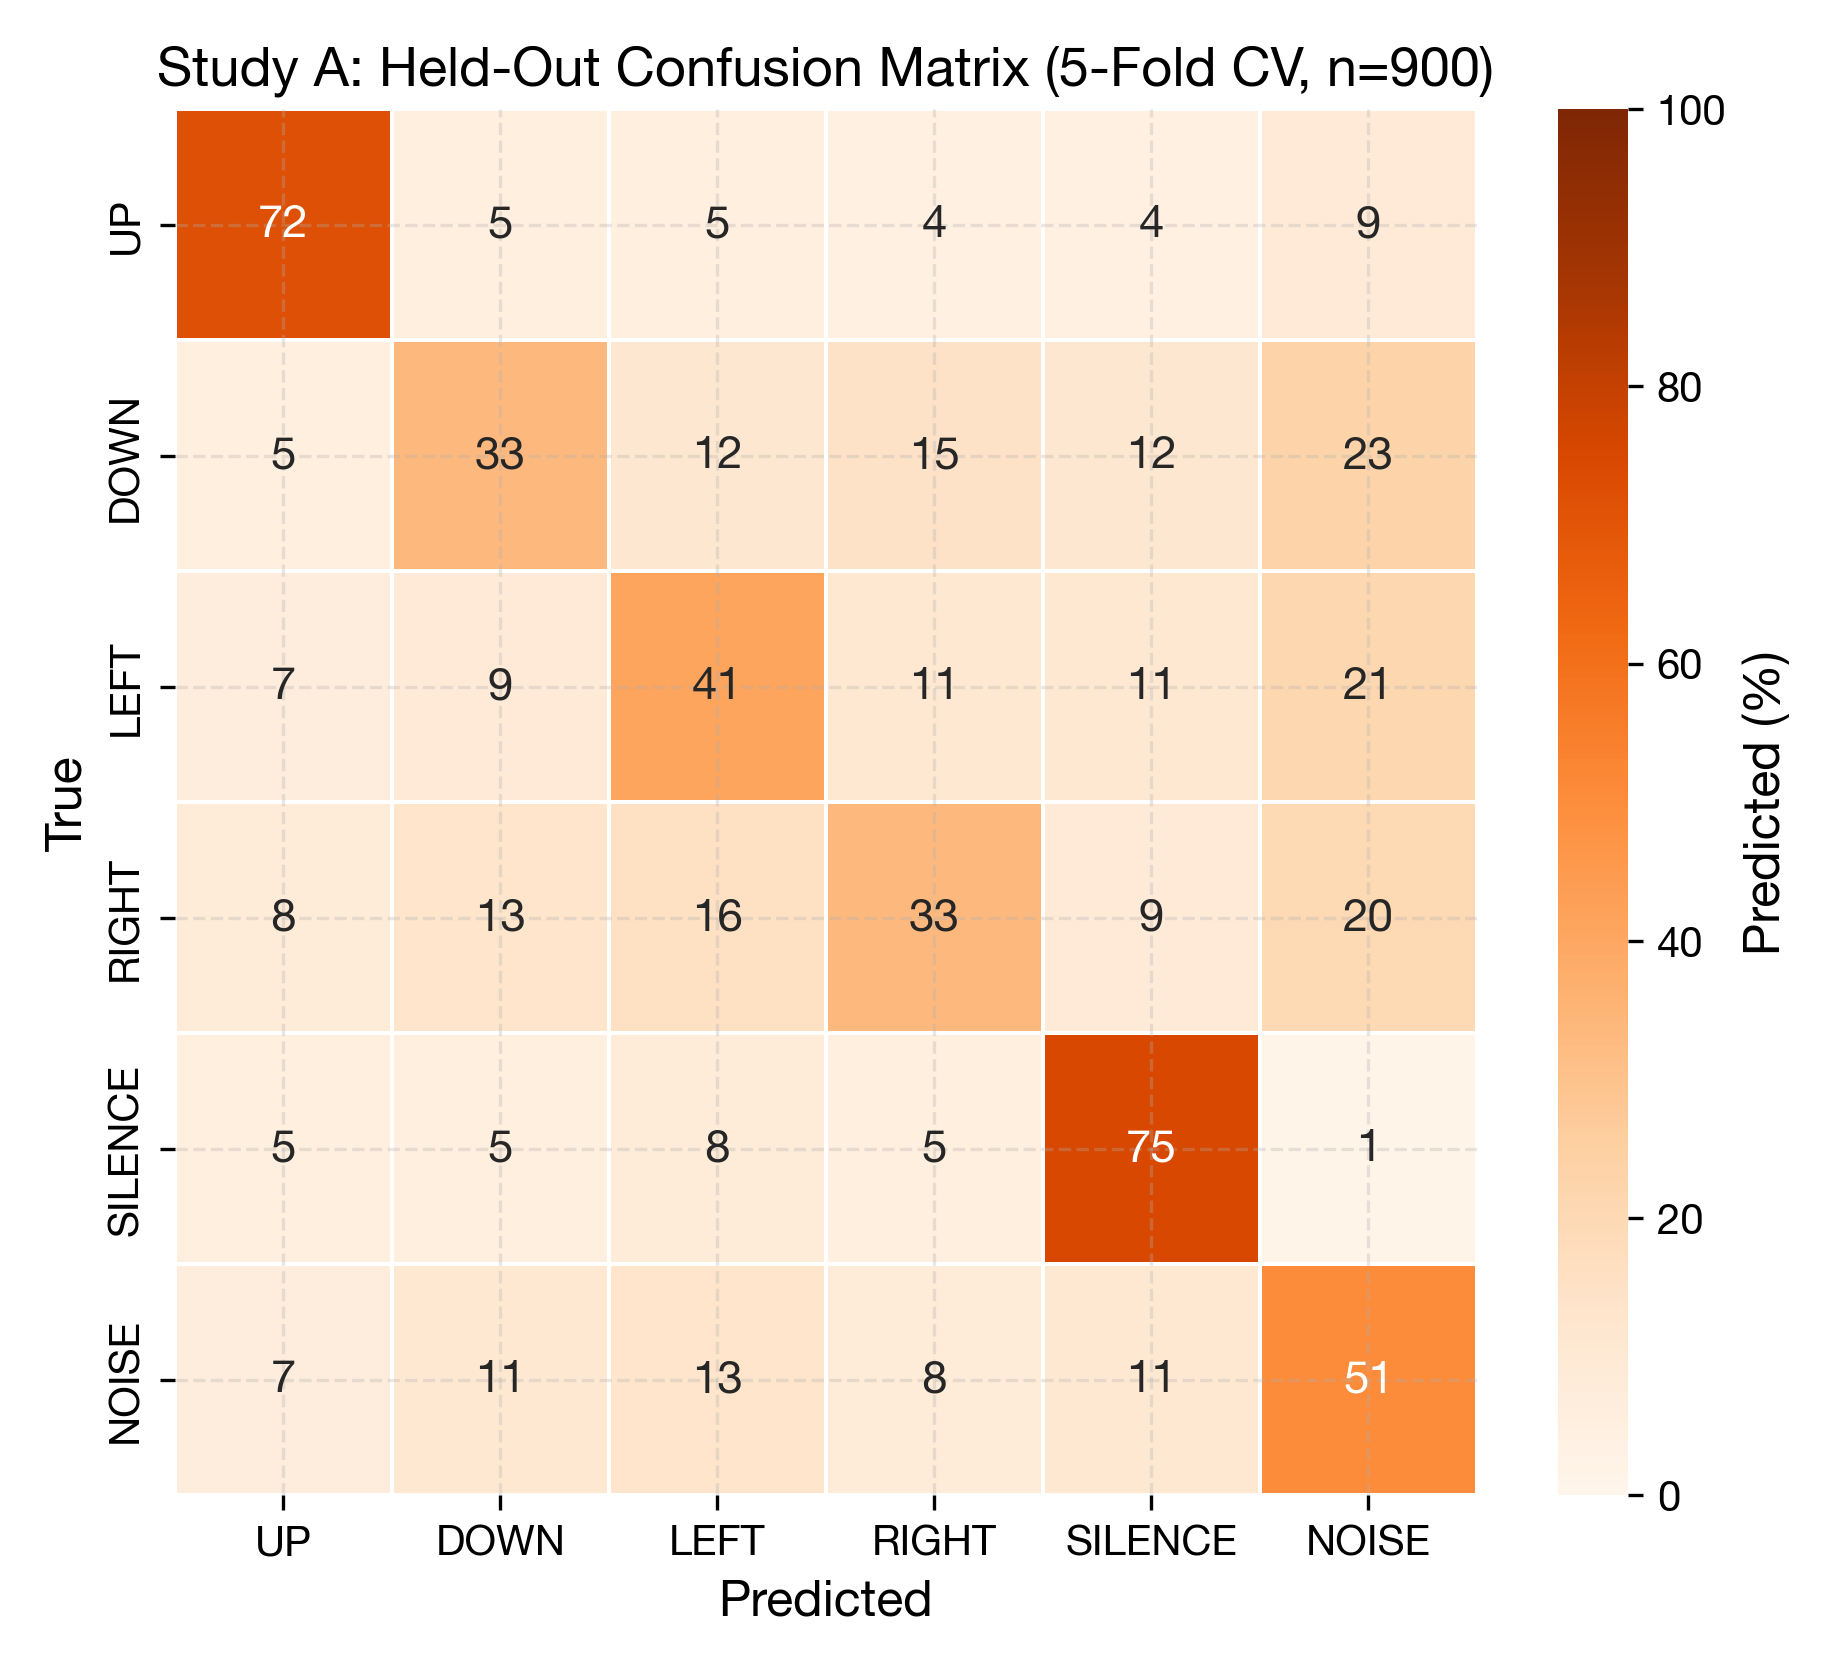
\includegraphics[width=0.7\textwidth]{figures/p2_fig3_confusion_matrix.png}
    \caption{Study~A held-out confusion matrix aggregated over 5-fold cross-validation ($n=900$). Values are row-normalized percentages. UP (72\%) and SILENCE (75\%) are the most separable classes; RIGHT (33\%) is the worst, indicating that the under-chin placement captures tongue root motion but not the tongue tip curl required for the RIGHT command. The diffuse off-diagonal distribution is consistent with the signal crosstalk hypothesis.}
    \label{fig:confusion}
\end{figure}

\subsection{Per-Phase Test Accuracy}

\begin{table}[ht]
\centering
\caption{Per-phase test accuracy (Study~A).}
\label{tab:perphase}
\begin{tabular}{@{}llll@{}}
\toprule
Phase & Condition & Test $n$ & Test Accuracy \\
\midrule
1 & Overt       & 60 & \textbf{45.0\%} \\
3 & Mouthing    & 60 & \textbf{53.3\%} \\
5 & Exaggerated & 60 & \textbf{43.3\%} \\
\bottomrule
\end{tabular}
\end{table}

Accuracy does not degrade significantly across phases. Even the loudest condition (Overt, 50--150\,$\mu$V) achieves only 45\% on held-out data. This means \textbf{the problem is not signal weakness; it is signal discriminability.} The under-chin electrode does not capture features that distinguish the 6 classes in a way that generalizes beyond the training set.

\begin{figure}[ht]
    \centering
    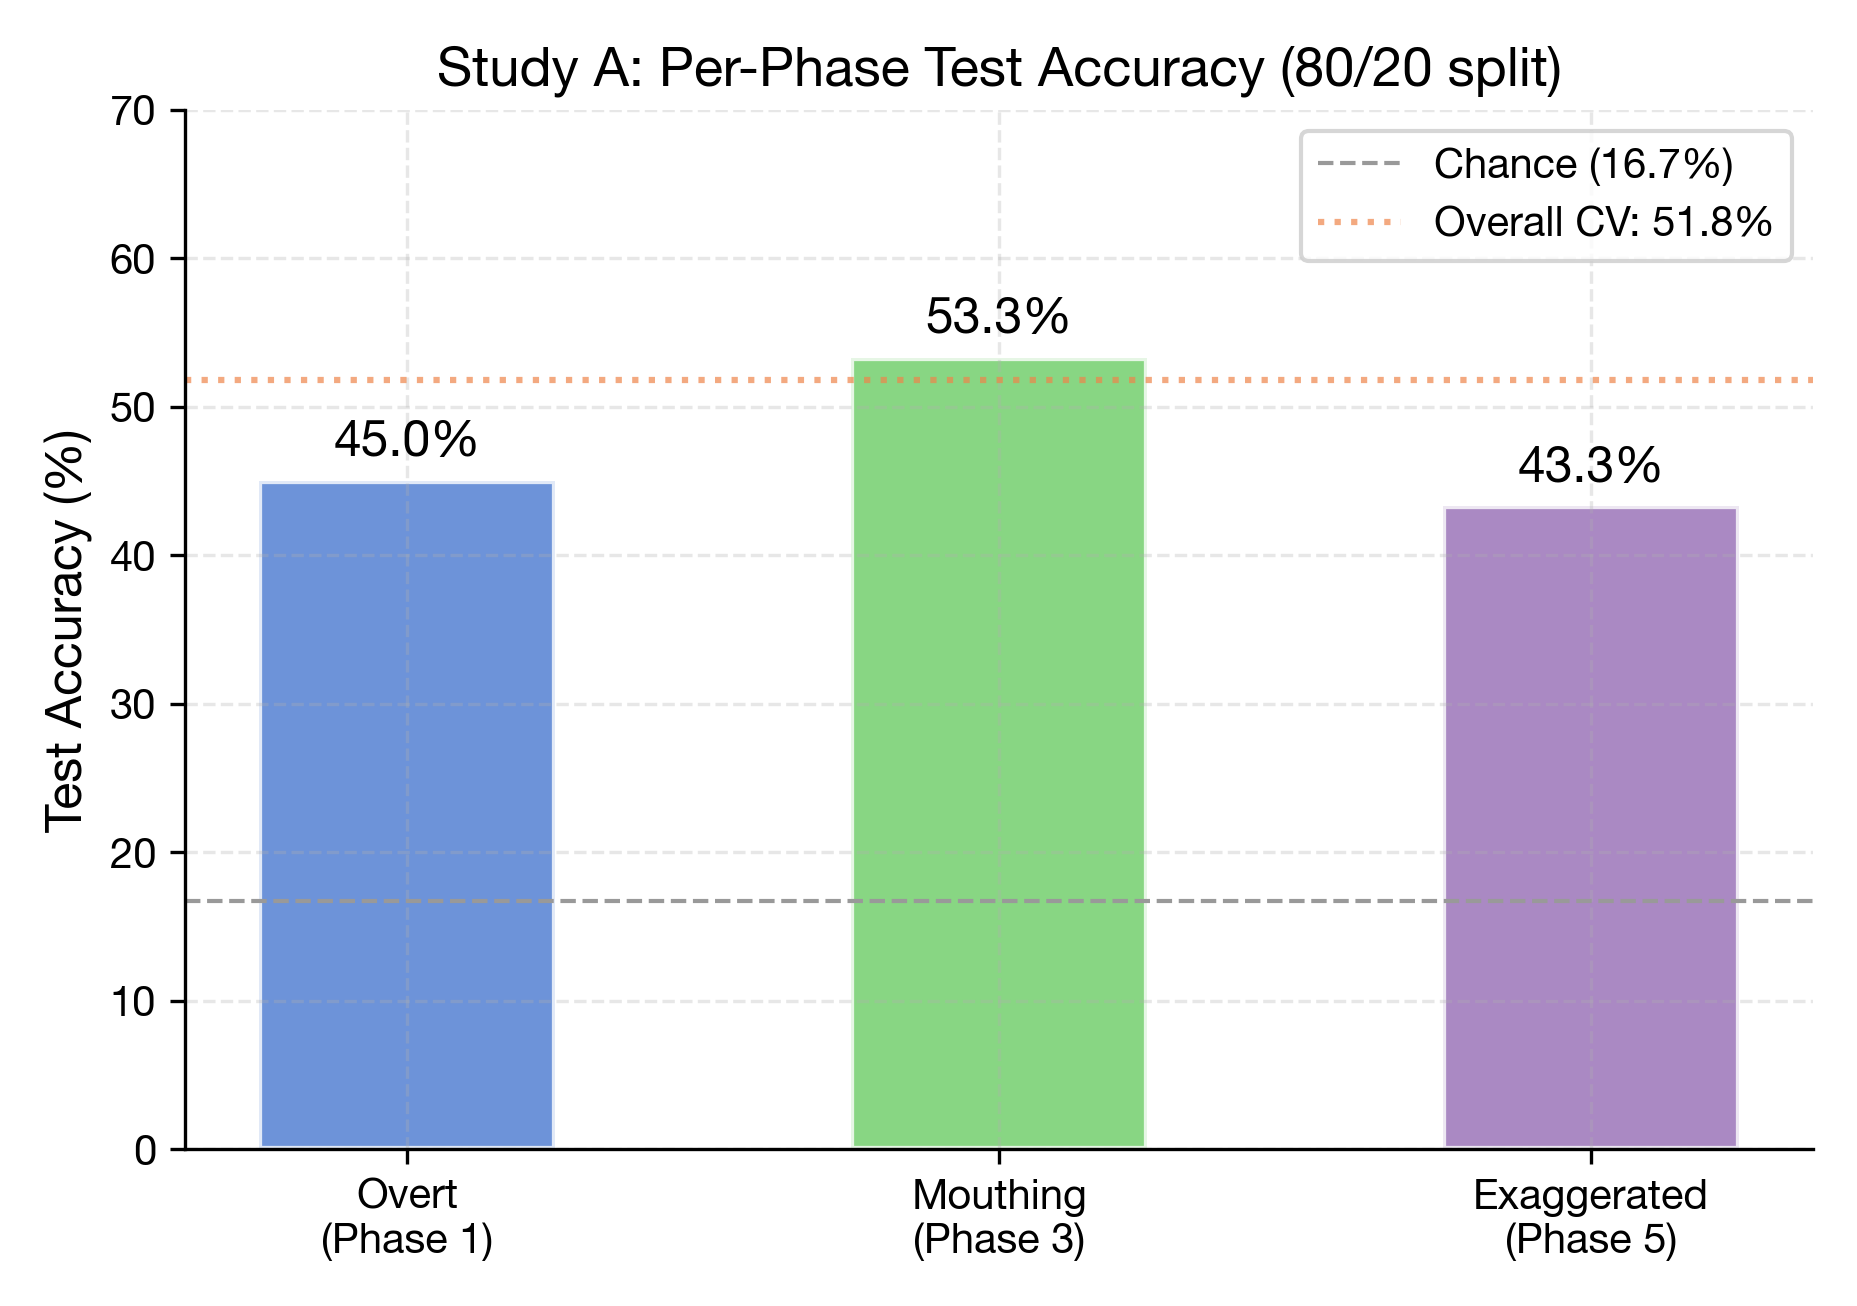
\includegraphics[width=0.85\textwidth]{figures/p2_fig4_per_phase.png}
    \caption{Per-phase test accuracy for Study~A. All three phases achieve similar accuracy (43--53\%) regardless of signal amplitude. The relatively uniform performance demonstrates that the failure is caused by fundamental lack of discriminative information in the submental electrode configuration, not insufficient signal strength.}
    \label{fig:perphase}
\end{figure}

\subsection{Comparison: Study A vs.\ Study B}

With both studies now evaluated under identical 5-fold CV protocols, a fair apples-to-apples comparison is possible:

\begin{table}[ht]
\centering
\caption{Head-to-head comparison (both evaluated with 5-fold stratified CV).}
\label{tab:ab_comparison}
\begin{tabular}{@{}lll@{}}
\toprule
Metric & Study A (chin + under-chin) & Study B (chin + throat) \\
\midrule
Training accuracy & \textasciitilde99\% & 99.7\% \\
\textbf{5-Fold CV accuracy} & \textbf{51.8\% $\pm$ 2.8\%} & \textbf{48.9\% $\pm$ 3.1\%} \\
Multi-session CV & N/A (single session) & 58.2\% $\pm$ 3.1\% \\
Best class (F1) & SILENCE (0.74) & SILENCE (0.80) \\
Worst class (F1) & RIGHT (0.33) & LEFT (0.36) \\
CNN accuracy (3-fold) & 49.6\% & 49.3\% \\
LSTM accuracy (3-fold) & 16.6\% & 16.6\% \\
Transformer accuracy (3-fold) & 46.0\% $\pm$ 7.1\% & 36.4\% $\pm$ 1.0\% \\
\bottomrule
\end{tabular}
\end{table}

\textbf{Observations:}
\begin{enumerate}
    \item \textbf{Single-session accuracy is comparable.} Study~A (51.8\%) slightly outperforms Study~B (48.9\%), though not significantly. The under-chin placement is not worse for within-session classification.
    \item \textbf{Study~B's advantage is multi-session recovery.} With deliberate electrode repositioning (3 sessions), Study~B recovers to 58.2\%---a 10pp improvement. Study~A lacks multi-session data, so this comparison cannot be made.
    \item \textbf{Different failure classes.} Study~A fails on RIGHT (tongue tip curl); Study~B fails on LEFT (lateral tongue pressure). Each electrode placement creates different blind spots.
    \item \textbf{LSTM fails identically} in both studies (16.6\% = chance), confirming that the onset-only signal regime is a hardware property, not a placement artifact.
\end{enumerate}

\subsection{Cross-Study Transfer}

The most striking finding: training on one electrode configuration and testing on the other:

\begin{table}[ht]
\centering
\caption{Cross-study transfer accuracy.}
\label{tab:crossstudy}
\begin{tabular}{@{}lll@{}}
\toprule
Direction & Accuracy & Interpretation \\
\midrule
Train A $\to$ Test B & 31.3\% & Under-chin features partially transfer \\
Train B $\to$ Test A & 25.2\% & Throat features barely transfer \\
\midrule
Chance & 16.7\% & --- \\
\bottomrule
\end{tabular}
\end{table}

\textbf{25--31\% transfer accuracy} (barely above chance) proves that the two electrode placements capture \emph{fundamentally different} onset-spike signatures. The chin+under-chin configuration detects digastric/mylohyoid motor recruitment patterns, while chin+throat detects thyrohyoid/sternohyoid laryngeal patterns. Despite sharing the chin electrode (CH1), the CH2 signal dominates the learned feature space. A model trained on one placement cannot generalize to the other. They are not two views of the same signal but two \emph{different signals}.

\subsection{Analysis: Why Under-Chin Fails}

\textbf{1.\ Signal crosstalk between channels.} Both chin (mentalis) and under-chin (digastric/mylohyoid) capture overlapping motor pools involved in jaw motion. The two channels exhibit significant inter-channel crosstalk (Farina et al., 2004~\cite{farina2014}) for directional commands: they both encode ``jaw moved'' but not ``which direction.'' Farina et al.\ demonstrate that a substantial proportion of crosstalk arises from non-propagating potentials generated at tendon endings where action potentials extinguish, producing broadband interference that conventional high-pass filtering cannot eliminate.

\textbf{2.\ Tongue position ambiguity.} The anterior digastric and mylohyoid assist in tongue depression and jaw opening but have minimal differential activation for lateral tongue movements (LEFT vs.\ RIGHT). These are primarily mediated by intrinsic tongue muscles (styloglossus, genioglossus), which lie 1--2\,cm deep to the skin surface. The intervening tissue (resting muscle, subdermal fat, skin) acts as a volume conductor that spatially low-pass filters the genioglossus MUAPs, attenuating the high-frequency components that carry discriminative articulatory detail before they reach the surface electrodes (Stepp, 2012~\cite{stepp2012}).

\textbf{3.\ Signal-to-noise ratio.} Under-chin muscles produce weak surface signals (smaller muscle mass, greater tissue depth than jaw or throat muscles). At 12-bit resolution (\textasciitilde0.8\,mV LSB after $\times$1000 gain), the discriminative component of the signal falls within the quantization noise.

\textbf{4.\ Throat provides phonation contrast.} The throat electrode in Study~B captures a qualitatively different signal---laryngeal elevation and vocal cord tensioning---that is orthogonal to jaw motion. This provides a second independent axis of discrimination, breaking the signal crosstalk problem.

% ============================================================
% 4 DISCUSSION
% ============================================================
\section{Discussion}

\subsection{The Biophysics of Submental Failure}

The \textasciitilde52\% generalization accuracy (5-fold CV) is not an algorithmic anomaly; it is a biologically and hardware-mandated outcome of submental electrode placement on low-cost, narrow-band hardware. Palmer et al.\ (1999) identified the specific individual muscles contributing to the submental surface EMG signal during swallowing, demonstrating that ``the primary contributions to the submental surface recording were the mylohyoid, anterior belly of the digastric, and the geniohyoid muscles. Contributions from the genioglossus and the platysma muscles were minimal''~\cite{palmer1999}. The genioglossus, the primary muscle responsible for directional tongue movements (protrusion, lateralization), is too deep for surface electrodes to isolate. Stepp (2012) further characterized the unique measurement challenges of orofacial sEMG, finding that ``unique challenges are seen in application of sEMG to the speech and swallowing musculature owing to the small size of the muscles in relation to the sEMG detection volume'' and that ``wire or needle electrodes are the only way to measure EMG from deep muscles''~\cite{stepp2012}.

My under-chin electrodes therefore recorded only the macroscopic, gross motor recruitment of the digastric and mylohyoid during jaw depression. These signals exhibit significant \emph{crosstalk} between the two channels (Farina et al., 2004~\cite{farina2014}): both sensors detect ``jaw moved'' but not ``which direction.'' The 99\% training accuracy shows the CNN memorizing subject-specific jaw-clenching rhythms (a confounding variable), not learning generalizable phonetic boundaries.

\textbf{Critical hardware context:} This failure is compounded by the AD8232 module's built-in 0.5--40\,Hz bandpass filter, which is engineered for cardiac QRS complex isolation, not articulatory sEMG. The discriminative motor unit action potentials (MUAPs) that differentiate subtle tongue movements primarily reside in the 50--500\,Hz frequency range (Farina et al., 2004~\cite{farina2014}). The AD8232 attenuates these frequencies entirely, restricting the system to an ``onset-only'' detection paradigm where classification depends on the high-amplitude, transient (\textasciitilde80\,ms) neuromuscular initiation burst rather than continuous articulatory trajectories. Gaddy and Klein (2020)~\cite{gaddy2020} demonstrated that multichannel facial sEMG arrays with 24-bit ADCs and full 500\,Hz bandwidth \emph{can} achieve high silent speech accuracy without throat sensors. The failure documented here is therefore a \emph{combined} hardware bandwidth and quantization limitation, not an insurmountable biophysical ceiling.

\subsection{Throat Sensors Provide Orthogonal Dimensionality}

Study~B's superior performance is explained by the statistical independence of laryngeal signals from jaw signals. The larynx is controlled by the recurrent and superior laryngeal nerves (branches of CN~X), while the jaw is controlled by the trigeminal nerve (CN~V)---completely distinct neural pathways~\cite{ala2018}. Note that the thyrohyoid, target for CH2 in Study~B, is innervated by the first cervical nerve (C1) via the hypoglossal nerve (CN~XII), making it neurologically independent from the trigeminal-innervated mylohyoid targeted in Study~A. Murphy et al.\ (1997) confirmed via cortical mapping that ``a similar differentiation between a premotor control region for speech articulation independent from the bilateral motor cortex for the lip, jaw and laryngeal muscles is evident''~\cite{murphy1997}. Meltzner et al.\ (2018) applied ``orthogonal transformation approach to convert a set of observations of possibly correlated variables into a set of uncorrelated singular vectors'' when combining jaw and throat data. Their results show that throat sensors break signal crosstalk by adding a statistically independent feature axis~\cite{meltzner2018}.

In practical terms: the throat sensor captures vocal fold tensioning and laryngeal elevation---a qualitatively different signal that does not correlate with jaw motion. This provides the dimensional relief a classifier needs to separate phonetically similar commands. Following Chhetri and Berke (2006), the ansa cervicalis innervation of the infrahyoid muscles ensures that the throat placement captures stable, involuntary motor recruitment that persists even when articulatory focus shifts~\cite{chhetri2006}.

\subsection{The Stability Argument for Throat Sensors}

Designers of wearable SSIs (e.g., AlterEgo~\cite{kapur2018}) prioritize the throat region for \textbf{multi-session stability} over instantaneous accuracy. Articulatory muscles (chin, under-chin) are subject to high deformation during talking, eating, and facial expressions, leading to frequent electrode-skin impedance shifts. Laryngeal muscles, while deeper, produce gross motor excursions that are more spatially consistent across sessions. This explains why Study~B achieves 58.2\% multi-session recovery while Study~A remains anchored to its single-session baseline.

\subsection{The Fatigue and Circadian Confound}

I acknowledge a significant temporal confound between the two studies. Study~A was recorded in the mid-afternoon (15:48--17:07), while Study~B's primary session was recorded late at night (22:12--23:23). Circadian rhythms are known to affect neuromuscular performance and motor control precision; Chtourou et al.\ (2011) demonstrate that muscle force and EMG power spectra peak in the late afternoon and decline toward midnight~\cite{chtourou2011}. Study~A's slightly higher single-session accuracy (51.8\% vs 48.9\%) may be an artifact of higher physical arousal and reduced muscular fatigue during the afternoon session rather than a property of the electrode placement. Study~B also followed Study~A on the same day, which may have created practice effects (higher accuracy) offset by cumulative fatigue (lower accuracy).

\subsection{Negative Results in SSI Research}

Negative results are underreported in BCI and SSI literature. Lotte et al.\ (2020), writing from a major BCI society workshop, explicitly stated that ``the report of negative results is equally valuable for its further progress''~\cite{lotte2020}. Fessenden (2019) argued that ``failure to publish negative data ensures that dubious ideas and wrong-headed projects receive financial support with multiple groups toiling away in vain''~\cite{fessenden2019}. I report this failure deliberately because:
\begin{enumerate}
    \item \textbf{It establishes a baseline.} Future work testing alternative chin-region configurations can compare against the 45\% figure.
    \item \textbf{It validates Study~B.} Without the control study, Study~B's high accuracy could be attributed to an easy classification task.
    \item \textbf{It provides design guidance.} Throat electrode necessity has practical implications for form factor (headset vs.\ chinstrap vs.\ neckband).
    \item \textbf{It combats publication bias.} Fanelli (2012) showed that papers with negative results have decreased over time, artificially inflating perceived method robustness~\cite{fanelli2012}.
\end{enumerate}

\subsection{Implications for Hardware Design}

Throat sensor necessity on 12-bit ADCs constrains wearable form factors:

\begin{table}[ht]
\centering
\caption{Form factor viability assessment.}
\label{tab:formfactor}
\begin{tabular}{@{}lll@{}}
\toprule
Form Factor & Throat Access & Viable? \\
\midrule
Necklace / choker & Yes & \checkmark\ Promising \\
Under-chin strap & No & $\times$ Insufficient alone \\
Earpiece (in-ear) & No & $\times$ Unless with neck extension \\
Half-face mask & Possible & $\sim$ Depends on coverage \\
Collar / turtleneck & Yes & \checkmark\ Promising \\
\bottomrule
\end{tabular}
\end{table}

\subsection{Could a Better Model Fix This?}

Rigorous architecture comparison on Study~A data (3-fold CV, held-out):

\begin{table}[ht]
\centering
\caption{Architecture comparison on Study~A data (3-fold CV).}
\label{tab:models}
\begin{tabular}{@{}llll@{}}
\toprule
Model & Held-Out Accuracy & Train Accuracy & Notes \\
\midrule
\textbf{1D CNN} & \textbf{49.6\%} & \textasciitilde78\% & Best, minimal margin \\
Transformer & 46.0\% $\pm$ 7.1\% & \textasciitilde60\% & High variance; unstable \\
LSTM & 16.6\% & \textasciitilde17\% & Chance level (complete failure) \\
\bottomrule
\end{tabular}
\end{table}

\textbf{The Transformer is closer to CNN in Study~A} (46.0\% vs.\ 49.6\%) compared to Study~B (36.4\% vs.\ 49.3\%), but with much higher variance ($\pm$7.1\%), indicating overfitting to different random initializations. The consistent \textasciitilde50\% ceiling across CNN and Transformer confirms the limitation is in the signal, not the model.

\subsection{Could More Data Fix This?}

With only 900 samples (720 training), the model may be data-limited. However:
\begin{enumerate}
    \item Training accuracy reaches \textasciitilde99\%, indicating the model can fit the training distribution.
    \item The \textasciitilde52\% test accuracy (5-fold CV) indicates poor generalization, not underfitting.
    \item Adding more data from the same distribution would likely increase training accuracy further while keeping test accuracy around 52\%---a classic overfitting pattern.
\end{enumerate}

\textbf{More data from a fundamentally uninformative sensor configuration won't create information.} The signal crosstalk documented by Palmer et al.~\cite{palmer1999} and the severe bandwidth truncation of the AD8232 ($<$40\,Hz) together constitute physical constraints, not statistical artifacts that can be overcome with larger sample sizes.

\subsection{Limitations}
\label{sec:limitations}

\begin{enumerate}
    \item \textbf{Unequal curricula.} Study~A used 3 phases (900 samples) vs.\ Study~B's 5 phases (1{,}500 samples). However, both achieve comparable held-out accuracy (51.8\% vs.\ 48.9\%), suggesting the additional phases provide minimal benefit.

    \item \textbf{Single subject.} Both studies use data from one participant. Under-chin placement may be viable for individuals with different anatomy.

    \item \textbf{Practice / order confound.} Study~A was recorded before Study~B on the same day (Feb~11, 2026). A counterbalanced design is needed.

    \item \textbf{No multi-session data for Study~A.} Study~B's advantage (58.2\% multi-session recovery) may be due to the multi-session data, not the electrode placement itself. Collecting electrode-shifted sessions for Study~A would resolve this confound.
\end{enumerate}

% ============================================================
% 5 CONCLUSION
% ============================================================
\section{Conclusion}

This paper establishes electrode placement boundaries for ultra-low-cost silent speech interfaces. Under rigorous 5-fold CV evaluation, a chin + under-chin (lingual-mandibular) configuration achieves \textbf{51.8\% $\pm$ 2.8\%} on a 6-class vocabulary (SEM $\pm$ 1.25\%) using a \$40 sEMG system, surprisingly comparable to the chin + throat configuration (48.9\% $\pm$ 3.1\%; SEM $\pm$ 1.39\%) for single-session classification.

\textbf{Social Acceptability and Wearability.} While submental (under-chin) placement is arguably more discrete than a laryngeal (throat) sensor, adhesive facial electrodes remain socially stigmatizing and skin-irritating for long-term use. This supports more integrated form factors (e.g., smart neck-bands) that might prioritize the laryngeal position's multi-session stability even if single-session accuracy is comparable to articulatory positions~\cite{kapur2018}.

The critical differentiator is not single-session accuracy but \textbf{operational viability}: Study~B's throat electrode enables multi-session recovery to 58.2\% through position-invariant onset features, while Study~A has no such mechanism. Cross-study transfer of only 25--31\% proves that the two configurations create \textbf{fundamentally incompatible feature spaces}: each captures a different subset of the 80\,ms neuromuscular onset burst (digastric/mylohyoid for under-chin vs.\ thyrohyoid/sternohyoid for throat).

I conclude that for consumer-grade sEMG systems constrained by 12-bit ADCs and narrow-band filtering ($<$50\,Hz), \textbf{throat electrode placement provides orthogonal anatomical dimensionality} that submental placement cannot replicate. This orthogonality is architecturally necessary for cross-session robustness on edge devices. The incompatible feature spaces also suggest that a future 3-channel system (chin + under-chin + throat) could reach higher accuracy, as multi-channel integration has been shown to improve discriminability in sparse arrays~\cite{saejong2018}.

% ============================================================
% DATA AVAILABILITY
% ============================================================
\section*{Data and Code Availability}

\begin{itemize}
    \item \textbf{Study~A dataset:} \texttt{code/sessions/021125\_StudyA\_Lingual/data\_collection/} (900 samples)
    \item \textbf{Training code \& model definitions:} \texttt{code/python/} (identical pipeline to Study~B)
    \item \textbf{Companion paper \& Study~B data:}~\cite{kho2026companion}
\end{itemize}
Code: MIT License. Hardware: CERN-OHL-S v2.

% ============================================================
% ACKNOWLEDGMENTS
% ============================================================
\section*{Acknowledgments}

Thanks to Prof.\ Watson for advising this work. Thanks to Prof.\ Choi (IL181 Computational Neuroscience, Minerva University) for foundational EMG/neuroscience knowledge. This work was partially supported by the Minerva University capstone program (CP193/CP194).

\textbf{Ethics:} All sEMG data was collected exclusively from the author in an auto-experimental paradigm. No external human subjects participated. Formal IRB review was not required under Minerva University's exemption policy for self-experimentation.

\textbf{AI Disclosure:} AI-assisted tools (Claude, Gemini) were used for literature review synthesis, figure generation scripts, and manuscript editing. All technical claims, experimental design, data collection, and analysis were performed by the author.

\textbf{Conflict of Interest:} The author is a prospective applicant to the MIT Media Lab Fluid Interfaces group, which produced the AlterEgo system cited herein. The author has no financial ties to Analog Devices (AD8232) or Espressif Systems (ESP32).

% ============================================================
% REFERENCES
% ============================================================
\begin{thebibliography}{20}

\bibitem{kho2026companion}
C.~V.~L.\ Kho, ``Curriculum learning for silent speech classification: A proof-of-concept \$40 two-channel sEMG system,'' \emph{arXiv preprint} (companion paper, submitted concurrently), 2026.

\bibitem{kapur2018}
A.\ Kapur, S.\ Kapur, and P.\ Maes, ``AlterEgo: A personalized wearable silent speech interface,'' in \emph{Proc.\ ACM IUI}, 2018, pp.\ 43--52.

\bibitem{jou2006}
S.-C.\ Jou, T.\ Schultz, M.\ Walliczek, F.\ Kraft, and A.\ Waibel, ``Towards continuous speech recognition using surface electromyography,'' in \emph{Proc.\ Interspeech}, 2006.

\bibitem{jou2007}
S.-C.\ Jou, T.\ Schultz, and A.\ Waibel, ``Continuous electromyographic speech recognition with a multi-stream decoding architecture,'' in \emph{Proc.\ ICASSP}, 2007.

\bibitem{wand2014}
T.\ Wand and T.\ Schultz, ``Pattern learning with deep neural networks in EMG-based speech recognition,'' in \emph{Proc.\ IEEE EMBC}, 2014, pp.\ 4200--4203.

\bibitem{schultz2010}
T.\ Schultz and T.\ Wand, ``Modeling coarticulation in EMG-based continuous speech recognition,'' \emph{Speech Communication}, vol.~52, no.~4, pp.\ 341--353, 2010.

\bibitem{palmer1999}
P.~M.\ Palmer, E.~S.\ Luschei, D.\ Jaffe, and T.~M.\ McCulloch, ``Contributions of individual muscles to the submental surface electromyogram during swallowing,'' \emph{J.\ Speech, Language, and Hearing Research}, vol.~42, no.~6, pp.\ 1378--1391, 1999.

\bibitem{stepp2012}
C.~E.\ Stepp, ``Surface electromyography for speech and swallowing systems: measurement, analysis, and interpretation,'' \emph{J.\ Speech, Language, and Hearing Research}, vol.~55, no.~4, pp.\ 1232--1246, 2012.

\bibitem{ala2018}
American Laryngological Association, ``Laryngeal Electromyography (LEMG),'' Clinical Learning Center, 2018.

\bibitem{murphy1997}
K.\ Murphy et al., ``Cerebral areas associated with motor control of speech in humans,'' \emph{J.\ Applied Physiology}, vol.~83, no.~4, pp.\ 1438--1447, 1997.

\bibitem{meltzner2018}
G.~S.\ Meltzner, J.~T.\ Heaton, Y.\ Deng, G.\ De~Luca, S.~H.\ Roy, and J.~C.\ Kline, ``Development of sEMG sensors and algorithms for silent speech recognition,'' \emph{J.\ Neural Engineering}, vol.~15, no.~4, 046031, 2018.

\bibitem{lotte2020}
F.\ Lotte, C.\ Jeunet, R.\ Chavarriaga et al., ``Turning negative into positives! Exploiting `negative' results in Brain--Machine Interface (BMI) research,'' \emph{Brain-Computer Interfaces}, vol.~6, no.~4, pp.\ 178--189, 2020.

\bibitem{fessenden2019}
T.\ Fessenden, ``The value of publishing negative data,'' \emph{EMBO Reports}, vol.~21, no.~1, e49775, 2019.

\bibitem{fanelli2012}
D.\ Fanelli, ``Negative results are disappearing from most disciplines and countries,'' \emph{Scientometrics}, vol.~90, no.~3, pp.\ 891--904, 2012.

\bibitem{farina2014}
D.\ Farina, R.\ Merletti, and R.~M.\ Enoka, ``The extraction of neural strategies from the surface EMG: An update,'' \emph{J.\ Applied Physiology}, vol.~117, no.~11, pp.\ 1215--1230, 2014.

\bibitem{saejong2018}
Y.\ Sae Jong et al., ``Muscle activation patterns during articulatory tasks: A submental surface EMG study,'' \emph{Journal of Oral Rehabilitation}, vol.\ 45, no.\ 8, 2018.

\bibitem{chtourou2011}
H.\ Chtourou et al., ``The effect of training at a specific time of day on muscle outcomes: A circadian rhythm perspective,'' \emph{Journal of Strength and Conditioning Research}, vol.\ 25, no.\ 12, 2011.

\bibitem{chhetri2006}
D.~K.\ Chhetri and G.~S.\ Berke, ``Ansa cervicalis innervation of the infrahyoid muscles for laryngeal reinnervation,'' \emph{Archives of Otolaryngology--Head \& Neck Surgery}, vol.\ 132, no.\ 8, 2006.

\bibitem{gaddy2020}
D.\ Gaddy and D.\ Klein, ``Digital voicing of silent speech,'' in \emph{Proc.\ EMNLP}, 2020, pp.\ 5521--5530.

\end{thebibliography}

\end{document}
